\documentclass[10pt,letterpaper]{article} 
\usepackage{tikz}
\usepackage{tools}
\usepackage{enumitem}
\usepackage{listings}
\lstset{language=Python}
%\lstset{frame=lines}
%\lstset{caption={Insert code directly in your document}}
\lstset{label={lst:code_direct}}
\lstset{basicstyle=\footnotesize}

%\usepackage{graphicx}‎‎
%\usefonttheme{serif}‎
%\usepackage{ptext}‎
%\usepackage{xepersian}
%\settextfont{B Nazanin}
\usepackage{lipsum}
\setlength{\parindent}{0pt}
\setlength{\parskip}{1em}
\newcommand{\pf}{$\blacksquare$}

\newcommand{\Span}{\text{Span}}
\newcommand{\NF}{\text{NF}}
\newcommand{\EDFA}{\text{EDFA}}
\newcommand{\ASE}{\text{ASE}}

\newcommand{\bns}{\textit{broadcast-and-select}  architecture}
\newcommand{\Bns}{\textit{Broadcast-and-select} architecture}

\newcommand{\rns}{\textit{route-and-select} architecture}
\newcommand{\Rns}{\textit{Route-and-select} architecture}

\newcommand{\red}[1]{{\color{red}#1}}

\newcounter{QuestionNumber}
\setcounter{QuestionNumber}{1}

\newcommand{\Q}{
\textbf{Question \theQuestionNumber)}
\stepcounter{QuestionNumber}
}
\newcommand{\EX}{\Bbb E}
\newcommand{\nl}{\newline\newline}
%\newcommand{\pic}[2]{
%\begin{center}
%\includegraphics[width=#2]{#1}
%\end{center}
%}
\begin{document}
\large
\begin{center}
In the name of beauty

The $2^\text{nd}$ simulation assignment of Optical Networks course
\hl
\end{center}
\section{Introduction}
The aim of this computer assignment is to get a feeling for how the performance of a digital binary optical communication link is affected by parameters characteristic for this kind of systems. In the provided simulation software (Matlab scripts available from the courses homepage) you can manipulate the bit rate, the modulation format, the extinction ratio, the dispersion etc.
You are expected to hand in a brief report of your work containing the conclusions you have reached, together with appropriate figures and explanations. In this computer assignment we will use the Q-value as qualifier of the transmission. The Q-value is a statistical measure which can be related to bit error rate (BER). By using the Q-value to estimate the BER instead of counting errors, it is possible to use shorter bit streams in the simulation, thus the computation time can be reduced. However, you still have to make sure that you use sufficiently many bits to make the Q-value converge and not vary too much from run to run. When you do the simulations you should use a carrier wavelength and a transmitter chirp based on personal information, namely your day of birth (in the interval [1, 31]). The operating wavelength is calculated by $\lambda_c$ = 1530 + day of birth [nm]. The chirp parameter, C, is given by your birthday according to the table below. The sign of the chirp should be negative and positive for even and odd birthdays, respectively.
\begin{table}[h]
\centering
\Large
\begin{tabular}{|c|c|}
\hline
Day of birth & Chirp parameter\\\hline
1-9&3\\\hline
10-19&2\\\hline
20-29&1\\\hline
30-31&0\\\hline
\end{tabular}
\end{table}

Example: A person born on the 14th should use a carrier wavelength of 1544 nm and a chirp of –2, whereas a person born the 15th should use wavelength 1545 nm and chirp +2.

Other parameters to be used are listed at the end. Some of the parameters are cannot be changed from the GUI. The GUI itself is described in a separate section below.

\section{Back-to-back}
\begin{enumerate}
\item
Consider a NRZ-modulated back-to-back system, i.e. the transmitter is coupled directly to the receiver via a variable attenuator. The receiver has no optical pre-amplification. Reduce the SNR by setting the variable attenuator at 15 dB. Find the optimum electrical filter bandwidth of the receiver. Provide a plot of versus filter bandwidth. Why is there an optimum filter bandwidth, i.e. what is causing the penalty for wider and narrower filters? Use the found optimal electrical filter bandwidth in the next task.
\item
What is the receiver sensitivity (defined as the average received power (given by the GUI) that gives a Q-value of 6, which corresponds to BER = $10^{-9}$)? Compare your received value with the theoretical value of the receiver sensitivity. Why do they differ?
\item
How is the optimum bandwidth altered when changing to RZ-pulses? Set the variable attenuator to 12 dB. Give an explanation to why this happens. (Choose RZ pulse width (FWHM) to be one third of the bit slot).
\item
Use an EDFA as an optical pre-amplifier without any optical filter. What receiver sensitivity can you reach now? Use NRZ-pulses for this task.
\item
Use the 1 nm optical filter in combination with the optical pre-amplifier and find the receiver sensitivity for this receiver. This receiver implementation also causes a significant change that can be observed in the eye-diagram and decision point histogram. Explain what has happened.
\end{enumerate}
\section{Transmission without dispersion compensation}
By checking the ``Transmission w/o disp. comp.'' button, standard SMF transmission fiber is added to the system. The length of the fiber and the number of fiber spans can be set arbitrarily in the program. (Please note that the last amplifier is located at the receiver acting as pre-amplifier. The received signal power is the signal power leaving the last SMF.)
\begin{enumerate}
\item
How far can you transmit data (BER = $10^{-9}$) if you are allowed to used as many EDFAs as desired? What is limiting the transmission distance? Do this for both 10 Gbit/s and 40 Gbit/s and compare the difference for NRZ and RZ modulated data (provide a table).
\item
Why is one of the modulation formats more sensitive to dispersion?
\end{enumerate}
\section{Transmission with dispersion compensation}
Dispersion can be compensated by using dispersion compensating fibers (DCFs), which have large dispersion with opposite sign of the dispersion compared to standard transmission fibers (Check the ``Transmission w/o disp. comp.'' button). The compensation is done by installing the appropriate length of DCF. Dispersion compensation is commonly installed for each amplifier span by using amplifier stages consisting of two EDFAs with DCF in between. (Please note that the last two amplifiers and DCF are located at the receiver. The received signal power is the signal power leaving the last SMF.)
Please note that the dispersion for SMF and DCF is given at $\lambda$ = 1550 nm and that the dispersion slopes has to be used when the optimum DCF length is calculated. This calculation should be shown in the brief report.
\begin{enumerate}
\item
How far can you transmit with 10 and 40 Gbit/s in the NRZ and RZ cases if you install this kind of dispersion compensation (optimized for your wavelength) if the system has spans of 120 km? What is limiting the transmission distance?
\item
Keep the transmission distances you found above but decrease the amplifiers spacing to 60 km (remember to adjust the dispersion compensation.) Why is there an improvement?
\item
In spite of the dispersion compensation, when looking at the eye-diagrams using 60 km spans we can see that the signal is distorted compared to the back-to-back case, and the distortion increases with transmission distance and bit rate. What is causing this? (Please note that nonlinear effects are not included in this simulation program).
\item
You are asked to design a 1200 km long NRZ transmission link with a throughput of 40 Gbit/s. What is most beneficial from an economical perspective; to install $1 \times 40$ Gbit/s channel or $4 \times 10$ Gbit/s channels? You can access the fiber each 60 km. Assume that the equipment cost is as follows:

Transmitter 10 Gbit/s: \$500 Receiver 10 Gbit/s: \$1000

Transmitter 40 Gbit/s: \$2000 Receiver 40 Gbit/s: \$3000

In-line EDFA: \$2000
\end{enumerate}

\section{The MATLAB script}
You need five files to run the simulation software. These are available as a zip archive from the course homepage and should be placed in the same directory. The program is started by typing ``opticaltransmissionGUI'' in the MATLAB command window. You will now get a graphical user interface (GUI) window to work with. (MATLAB GUIs cannot be resized.) You can change various parameters and system settings to solve the assignment. Important readouts are the -value and the received power at the lower center of the window. Note also the sliders next to the figure which set the decision point in the eye-diagram. The histogram figure is extracted at the decision time indicated by the red dashed lines. The figure to the right plots the signal spectrum with and/or without electrical filter to visualize the influence of the filter.
\begin{figure}[h]
\centering
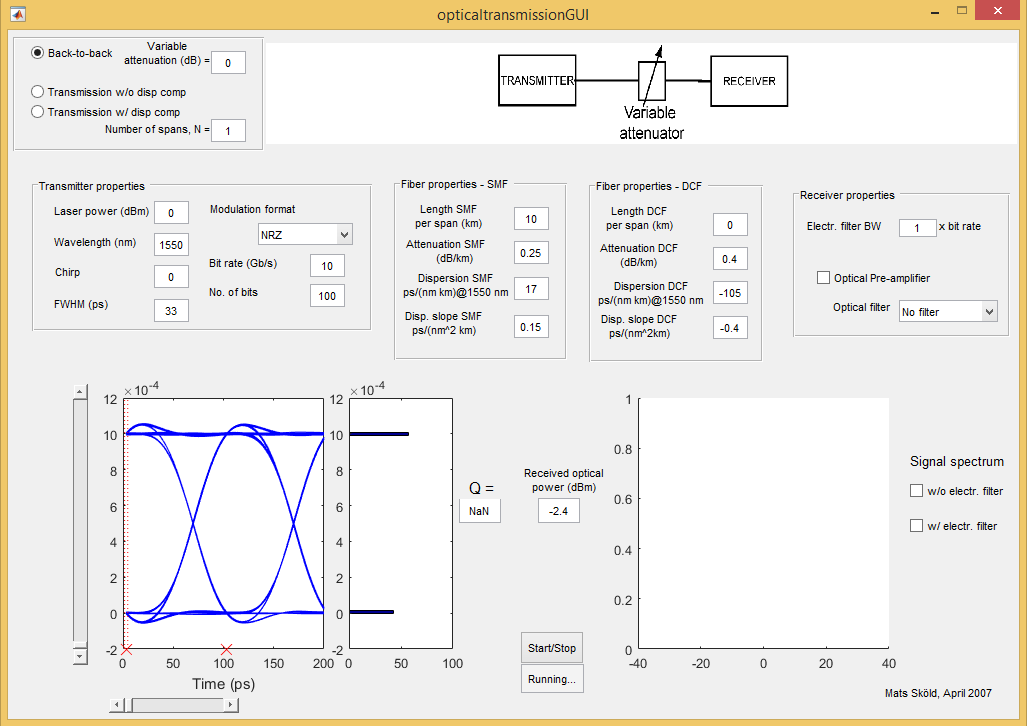
\includegraphics[width=160mm]{back2back_example}
\caption{An illustration of back-to-back system simulation}
\end{figure}
\section{Hints}
\begin{itemize}
\item
Use the slide bars to optimize the decision point. You must change this if the eye-diagram changes so you always make decisions at the optimal point!
\item
Remember to check that your values are reasonable! A Q-value of e.g. 100 is NOT reasonable.
\item
'Alt+print screen' generates a copy of the active window (in Windows) to the clipboard. Could be useful for the report.
\item
The dispersion compensation fibers are not considered to contribute to the overall transmission distance, since they are installed together with amplifiers at access points of the transmission fiber.
\item
Please provide the calculations that you have done and explanations to all figures and obtained results. A copied figure from the simulation program without explanation is not a good answer. Remember that this home assignment should be handed in as a brief report.
\end{itemize}
\section{Parameters}
\begin{table}[h]
\centering
\Large
\begin{tabular}{|l|c|}
\hline
SMF attenuation ($\alpha_\text{SMF}$)&0.25dB/km\\\hline
DCF attenuation ($\alpha_\text{DCF}$)&0.4dB/km\\\hline
SMF dispersion parameter at 1550nm ($D_\text{SMF}$)&17ps/nm/km\\\hline
SMF dispersion slope at 1550nm ($S_\text{SMF}$)&0.15 ps/$\text{nm}^2/\text{km}$\\\hline
DCF dispersion parameter at 1550nm ($D_\text{DCF}$)&-105ps/nm/km\\\hline
DCF dispersion slope at 1550nm ($S_\text{DCF}$)&0.4 ps/$\text{nm}^2/\text{km}$\\\hline
Transmitter max. optical output power ($P_{\text{tr},\text{max}}$)&6dBm\\\hline
Transmitter extinction ratio&0\\\hline
Receiver responsivity, RD&1 A/W\\\hline
Receiver load resistance,&$300\Omega$\\\hline
Receiver electr. filter order (Butterworth filter)&3\\\hline
Receiver Noise Figure&4 dB\\\hline
\end{tabular}
\end{table}
\end{document}